\documentclass{article}

\usepackage{tikz}

 

\begin{document}

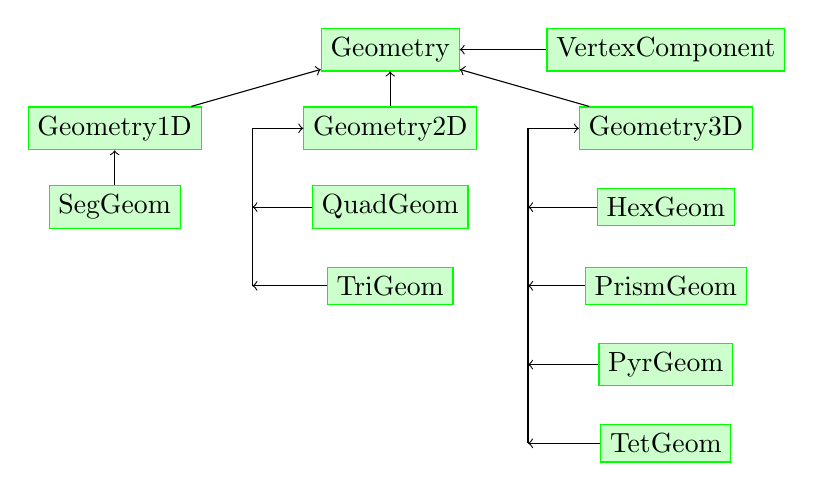
\begin{tikzpicture}[outline/.style={draw=#1,fill=#1!20}]

%NODES


\node [outline=green] (Geometry)                                   at (3.5,0)          {Geometry};
\node [outline=green] (VertexComponent)                                   at (7,0)          {VertexComponent};


\node [outline=green] (Geometry1D)                              at (0,-1)        {Geometry1D};
\node [outline=green] (Geometry2D)                              at (3.5,-1)        {Geometry2D};
\node [outline=green] (Geometry3D)                              at (7,-1)        {Geometry3D};

\node [outline=green] (SegGeom)                    at (0,-2)         {SegGeom};
\node [outline=green] (QuadGeom)                    at (3.5,-2)         {QuadGeom};
\node [outline=green] (TriGeom)                    at (3.5,-3)         {TriGeom};

\node [outline=green] (HexGeom)                    at (7,-2)         {HexGeom};
\node  [outline=green](PrismGeom)              at (7,-3)         {PrismGeom};
\node [outline=green] (PyrGeom)                    at (7,-4)         {PyrGeom};
\node [outline=green] (TetGeom)                    at (7,-5)         {TetGeom};

%CONNECTIONS

\draw[<-] (Geometry2D)--(1.75,-1);

\draw (1.75,-2) -- (1.75,-1) ;
\draw[<-] (1.75,-2)--(QuadGeom);

\draw (1.75,-3) -- (1.75,-2) ;
\draw[<-] (1.75,-3)--(TriGeom);


\draw[<-] (Geometry3D)--(5.25,-1);

\draw (5.25,-2) -- (5.25,-1) ;
\draw[<-] (5.25,-2)--(HexGeom);

\draw (5.25,-3) -- (5.25,-2) ;
\draw[<-] (5.25,-3)--(PrismGeom);

\draw (5.25,-4) -- (5.25,-3) ;
\draw[<-] (5.25,-4)--(PyrGeom);

\draw (5.25,-5) -- (5.25,-4) ;
\draw[<-] (5.25,-5)--(TetGeom);

\path[<-]  (Geometry)      edge (Geometry1D)
                 (Geometry)      edge (Geometry2D)
                 (Geometry)      edge (Geometry3D)
                 (Geometry)      edge (VertexComponent)
                 (Geometry1D)      edge (SegGeom);
\end{tikzpicture}


\end{document}